\documentclass[]{article}
\usepackage{lmodern}
\usepackage{amssymb,amsmath}
\usepackage{ifxetex,ifluatex}
\usepackage{fixltx2e} % provides \textsubscript
\ifnum 0\ifxetex 1\fi\ifluatex 1\fi=0 % if pdftex
  \usepackage[T1]{fontenc}
  \usepackage[utf8]{inputenc}
\else % if luatex or xelatex
  \ifxetex
    \usepackage{mathspec}
  \else
    \usepackage{fontspec}
  \fi
  \defaultfontfeatures{Ligatures=TeX,Scale=MatchLowercase}
\fi
% use upquote if available, for straight quotes in verbatim environments
\IfFileExists{upquote.sty}{\usepackage{upquote}}{}
% use microtype if available
\IfFileExists{microtype.sty}{%
\usepackage{microtype}
\UseMicrotypeSet[protrusion]{basicmath} % disable protrusion for tt fonts
}{}
\usepackage[margin=1in]{geometry}
\usepackage{hyperref}
\hypersetup{unicode=true,
            pdftitle={NestZModels},
            pdfborder={0 0 0},
            breaklinks=true}
\urlstyle{same}  % don't use monospace font for urls
\usepackage{graphicx,grffile}
\makeatletter
\def\maxwidth{\ifdim\Gin@nat@width>\linewidth\linewidth\else\Gin@nat@width\fi}
\def\maxheight{\ifdim\Gin@nat@height>\textheight\textheight\else\Gin@nat@height\fi}
\makeatother
% Scale images if necessary, so that they will not overflow the page
% margins by default, and it is still possible to overwrite the defaults
% using explicit options in \includegraphics[width, height, ...]{}
\setkeys{Gin}{width=\maxwidth,height=\maxheight,keepaspectratio}
\IfFileExists{parskip.sty}{%
\usepackage{parskip}
}{% else
\setlength{\parindent}{0pt}
\setlength{\parskip}{6pt plus 2pt minus 1pt}
}
\setlength{\emergencystretch}{3em}  % prevent overfull lines
\providecommand{\tightlist}{%
  \setlength{\itemsep}{0pt}\setlength{\parskip}{0pt}}
\setcounter{secnumdepth}{0}
% Redefines (sub)paragraphs to behave more like sections
\ifx\paragraph\undefined\else
\let\oldparagraph\paragraph
\renewcommand{\paragraph}[1]{\oldparagraph{#1}\mbox{}}
\fi
\ifx\subparagraph\undefined\else
\let\oldsubparagraph\subparagraph
\renewcommand{\subparagraph}[1]{\oldsubparagraph{#1}\mbox{}}
\fi

%%% Use protect on footnotes to avoid problems with footnotes in titles
\let\rmarkdownfootnote\footnote%
\def\footnote{\protect\rmarkdownfootnote}

%%% Change title format to be more compact
\usepackage{titling}

% Create subtitle command for use in maketitle
\newcommand{\subtitle}[1]{
  \posttitle{
    \begin{center}\large#1\end{center}
    }
}

\setlength{\droptitle}{-2em}
  \title{NestZModels}
  \pretitle{\vspace{\droptitle}\centering\huge}
  \posttitle{\par}
  \author{}
  \preauthor{}\postauthor{}
  \date{}
  \predate{}\postdate{}


\begin{document}
\maketitle

\begin{verbatim}
##  [1] "X"                "Site"             "Alt_m"           
##  [4] "Area_ha"          "Perim_m"          "Easting"         
##  [7] "Northing"         "No.of.Des"        "Any.Anc"         
## [10] "Pos_Hetero_Index" "Buffer1"          "Buffer2"         
## [13] "Buffer3"          "Richness"         "no_NVC"          
## [16] "sd_pH"            "sd_SOM"           "no_MSG"          
## [19] "sd_LBA"           "sd_meandbh"       "sd_treedensity"  
## [22] "no_trees"         "sd_R"             "mean_R"          
## [25] "sd_N"             "mean_N"           "sd_W"            
## [28] "mean_W"           "sd_L"             "mean_L"          
## [31] "meandbh"          "meanph"           "meanSOM"         
## [34] "meanLBA"          "meantreedensity"  "area_ratio"
\end{verbatim}

\begin{verbatim}
## Joining, by = "Site"
\end{verbatim}

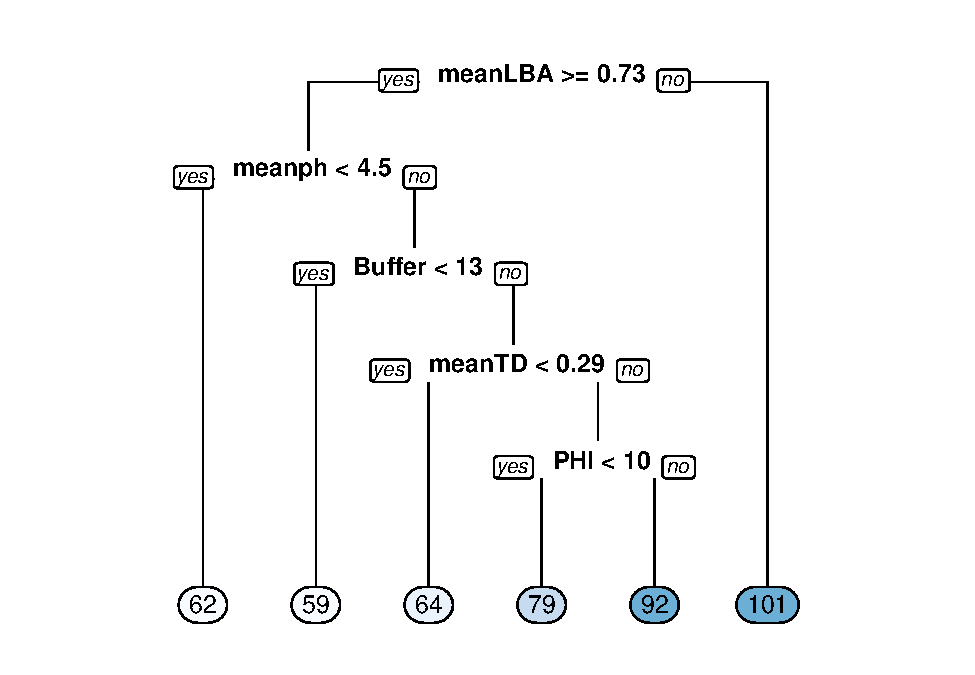
\includegraphics{NestZModels_files/figure-latex/unnamed-chunk-4-1.pdf}

\begin{verbatim}
##            round(apply(SitedataZ[-c(1, 14)], 2, function(x) dcor(x, SitedataZ$slope)), digits = 2)
## PHI                                                                                           0.38
## Buffer                                                                                        0.20
## Num_NVC                                                                                       0.21
## sd_pH                                                                                         0.12
## sd_SOM                                                                                        0.16
## sd_LBA                                                                                        0.16
## sd_meanDBH                                                                                    0.14
## meanDBH                                                                                       0.16
## meanph                                                                                        0.21
## meanSOM                                                                                       0.19
## meanLBA                                                                                       0.14
## area_ratio                                                                                    0.16
\end{verbatim}

The two varibles with the lowest correlation coefficients (dcor distance
correlation) to slope are number of major soil groups and mean tree
density,(Corr = 0.12,0.11) The number of major soil groups was included
since it might relfect habitat heterogeneity. However, its effect on
species richness is not clear here. It may change the species
assemblage, but not influence richness. This variable will be removed.
Mean tree density would be expected to affect richness as loewr density
would allow additional species with higher L values. But the low
correlation, and the fact that sd of tree density as well as mean dbh
are still included supports the removal of this variable.

The outliers in PHI, area\_ratio and sd\_SOM make it had to see the
reponse of slope to these variable. Initially I removed some outliers,
but the distribution of some variables, eg sd\_SOM was very right skew,
therefore decided to look at log fit instead.

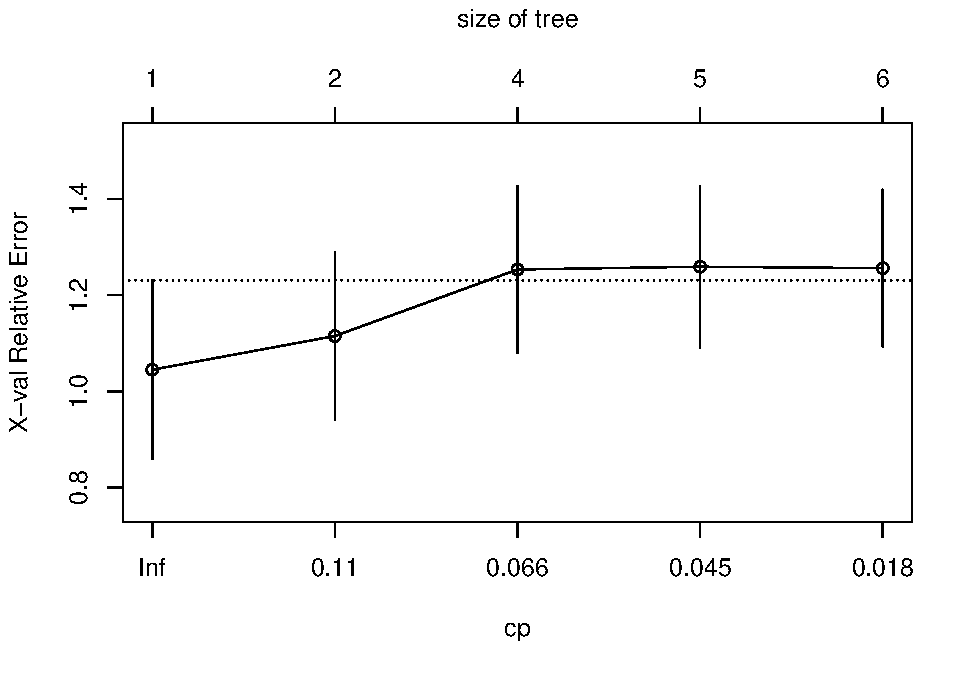
\includegraphics{NestZModels_files/figure-latex/unnamed-chunk-6-1.pdf}

\begin{verbatim}
##            slopecor
## PHI            0.42
## Buffer         0.21
## Num_NVC        0.20
## meanph         0.20
## meanSOM        0.18
## area_ratio     0.16
## sd_SOM         0.15
## sd_LBA         0.15
## sd_meanDBH     0.15
## meanDBH        0.15
## meanLBA        0.15
## sd_pH          0.12
\end{verbatim}

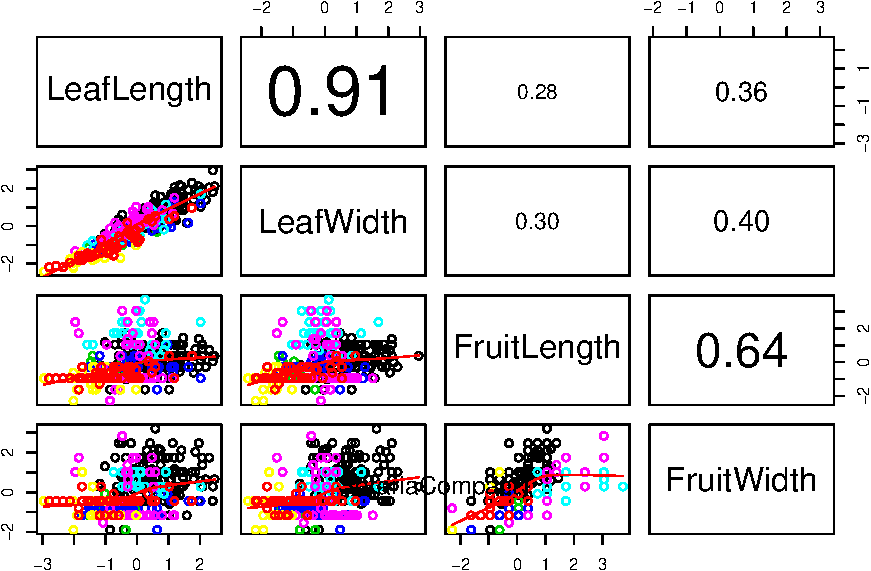
\includegraphics{NestZModels_files/figure-latex/unnamed-chunk-8-1.pdf}

\includegraphics{NestZModels_files/figure-latex/unnamed-chunk-9-1.pdf}

\includegraphics{NestZModels_files/figure-latex/unnamed-chunk-10-1.pdf}
\includegraphics{NestZModels_files/figure-latex/unnamed-chunk-11-1.pdf}
using either pearson or kendal correlations (even having removed
outliers which migh influence the pearson correlation) there are
correlations above 0.4 between the means and sd. Splitting the data into
two groups to separate these variables might give a less correlated set
of variables.

\section{Splitting the data into sd and
means}\label{splitting-the-data-into-sd-and-means}

\includegraphics{NestZModels_files/figure-latex/unnamed-chunk-13-1.pdf}
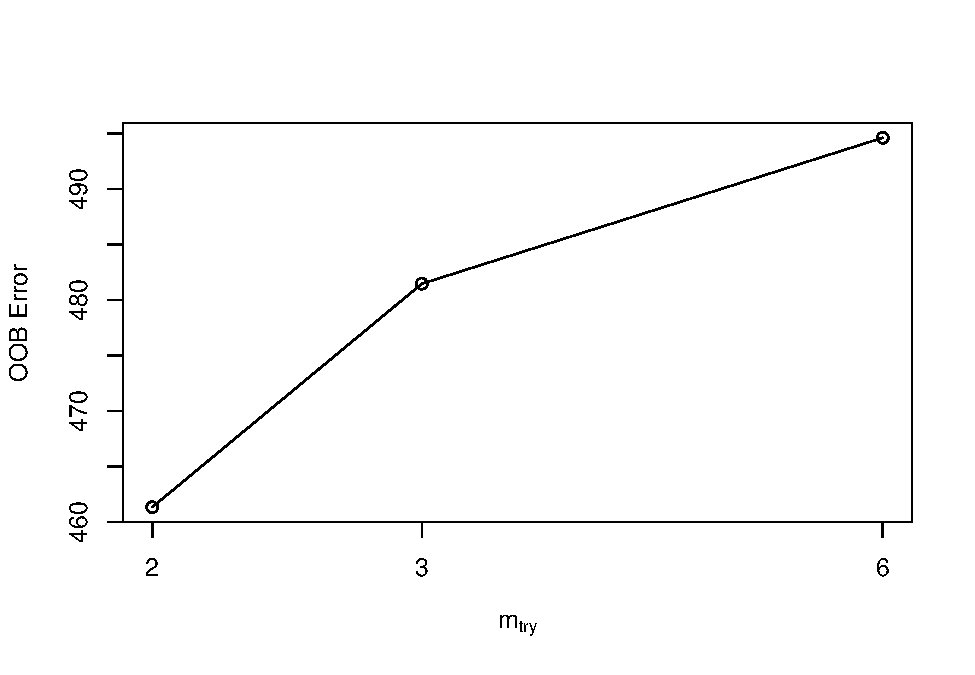
\includegraphics{NestZModels_files/figure-latex/unnamed-chunk-14-1.pdf}
The oearson method shows correaltion between sbuffer, and sd of SOM and
meandbh. The kendall does not show any correlations above 0.25. This may
be due to the outliers in SOM and mean DBH which are influencing the
pearson calculation.

\begin{verbatim}
##            slopecor
## PHI            0.42
## Buffer         0.21
## Num_NVC        0.20
## area_ratio     0.16
## sd_SOM         0.15
## sd_LBA         0.15
## sd_meanDBH     0.15
## sd_pH          0.12
\end{verbatim}

\begin{verbatim}
##            slopecor
## PHI            0.42
## Buffer         0.21
## Num_NVC        0.20
## meanph         0.20
## meanSOM        0.18
## area_ratio     0.16
## meanDBH        0.15
## meanLBA        0.15
\end{verbatim}

Both sets show a correlation (distance using dcor) of 0.42 with PHI with
the remaning correlations between the vars and slope being very similar.
The selection of variables could all potnetialy have an effect on
richness. This model analysis is lookin at the slope of the SAC from the
ln/ln lme model. This model can be thought of as an ``averaging'' effect
of the alpha diversity of each plot in the site. The effect of any
environmental variables on the slope at this scale should therefore be
small compared to the effect of the increasing area

\section{Models}\label{models}

\includegraphics{NestZModels_files/figure-latex/unnamed-chunk-17-1.pdf}

There is slight lack of linerity in the residuals plot due to one
outlier. The residuals do not apear to deviate substantially from
normality. Site 23 (point 78) appears to be influential - this is the
outlier in PHI

\begin{verbatim}
## Fixed term is "(Intercept)"
\end{verbatim}

\begin{verbatim}
## $`242`
## 
## Call:
## lm(formula = slope ~ area_ratio + meanph + meanSOM + Num_NVC + 
##     PHI + 1, data = data, na.action = "na.fail")
## 
## Coefficients:
## (Intercept)   area_ratio       meanph      meanSOM      Num_NVC  
##   0.2854521    0.0001995   -0.0121737   -0.0018080    0.0079558  
##         PHI  
##   0.0017081  
## 
## 
## $`241`
## 
## Call:
## lm(formula = slope ~ meanph + meanSOM + Num_NVC + PHI + 1, data = data, 
##     na.action = "na.fail")
## 
## Coefficients:
## (Intercept)       meanph      meanSOM      Num_NVC          PHI  
##    0.306006    -0.012730    -0.001613     0.007396     0.001679  
## 
## 
## attr(,"rank")
## function (x) 
## do.call("rank", list(x))
## <environment: 0x0000000017b64980>
## attr(,"rank")attr(,"call")
## AICc(x)
## attr(,"rank")attr(,"class")
## [1] "function"     "rankFunction"
## attr(,"beta")
## [1] "none"
\end{verbatim}

\begin{verbatim}
## Global model call: lm(formula = slope ~ ., data = data, na.action = "na.fail")
## ---
## Model selection table 
##      (Int)   are_rat       Bff      mnp       mSO  Num_NVC      PHI df
## 242 0.2855 0.0001995           -0.01217 -0.001808 0.007956 0.001708  7
## 241 0.3060                     -0.01273 -0.001613 0.007396 0.001679  6
## 177 0.3385                     -0.01185 -0.001637          0.001618  5
## 178 0.3226 0.0001748           -0.01131 -0.001810          0.001639  6
## 226 0.2183 0.0002161                    -0.001569 0.007372 0.001668  6
## 243 0.2995           9.982e-05 -0.01204 -0.001671 0.007424 0.001681  7
##      logLik   AICc delta weight
## 242 146.079 -277.0  0.00  0.286
## 241 144.872 -276.9  0.11  0.271
## 177 143.072 -275.5  1.45  0.138
## 178 143.971 -275.1  1.91  0.110
## 226 143.904 -274.9  2.05  0.103
## 243 144.933 -274.7  2.29  0.091
## Models ranked by AICc(x)
\end{verbatim}

The ``best'' two models use number NVC, meanpH, meanSOM, PHI and either
do or do not include area\_ratio. We expect meanSOM to effect pH, and
that pH effects richness, with greatest richness occurring around
neutral pH - so I am not sure why we would also include meanpHas well as
meanSOM. We are looking at slope of SAC across nests, not R of the
nests, but the greater the slope, the greater the richness of the nest.

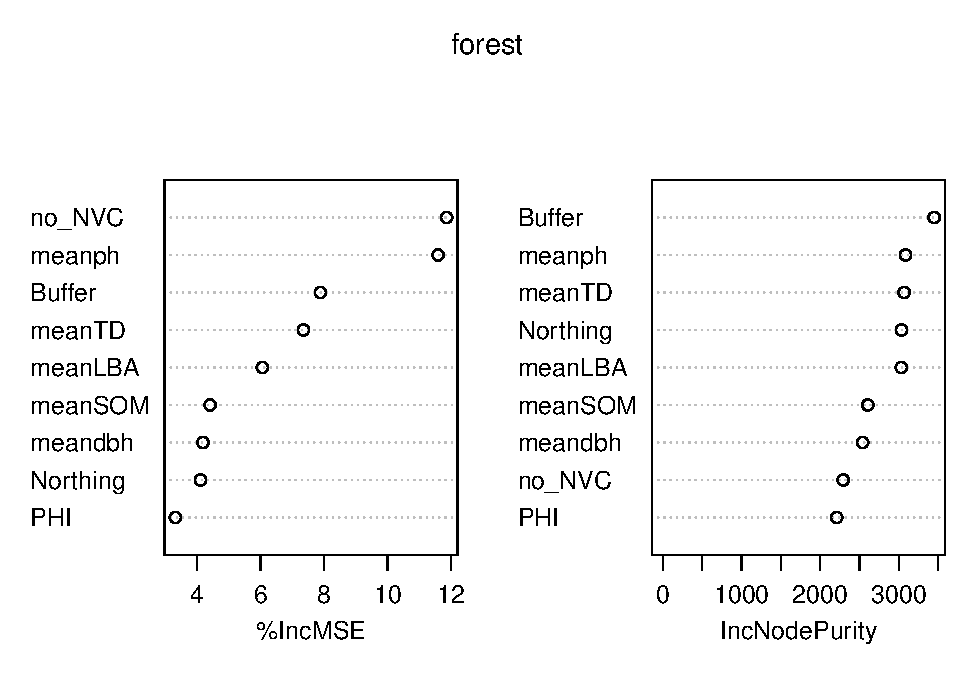
\includegraphics{NestZModels_files/figure-latex/unnamed-chunk-20-1.pdf}

The plots suggest that in these sites meanSOM is not strongly correlated
with meanpH at Site level, but at plot level there is a negative
correlation below pH5, However, there is a lot of scatter.

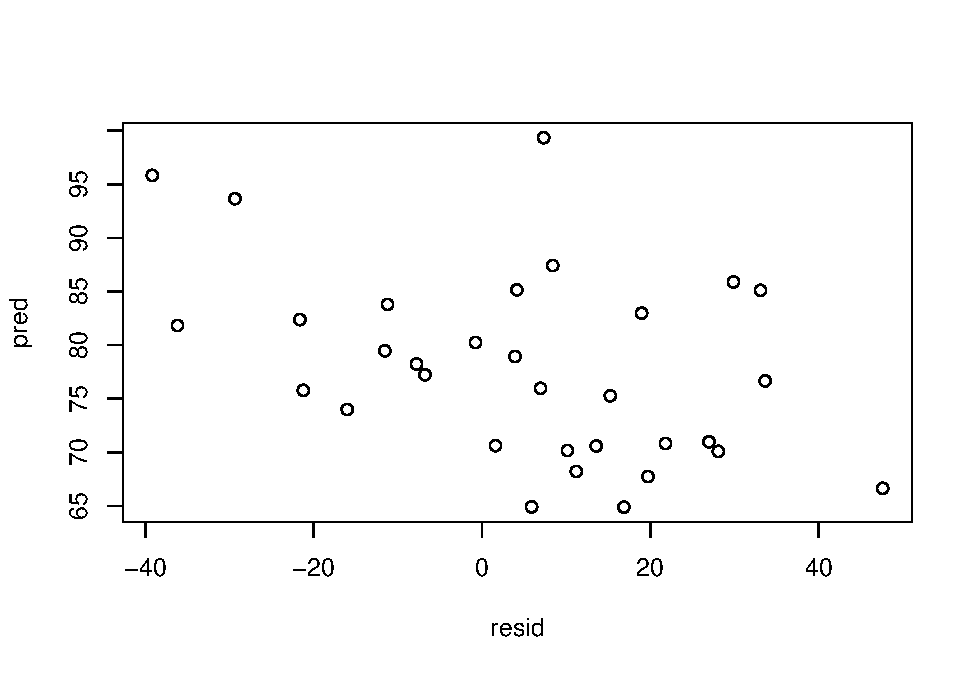
\includegraphics{NestZModels_files/figure-latex/unnamed-chunk-21-1.pdf}
The richness at site and plot level does not have a strong linear
correlation with pH, there is the expected unimodal peak, which is
stronger at site level. This would suggest that pH is s strong
influencing factor on richness, and thereby z, but its effect is not
linear. Therefore the coefficient of the linear term in the model could
be expected to be small and less signiicant than a non-linear term.

The richness as site or plot level does not appear to correlate strongly
with SOM, and its effect on the slope would therefore be small

These plots suggest that meanpH would be a bettter term for predictung
richness and therefore slope, but that it should be non-linear.


\end{document}
